% Drawing 154/08-17 -- folder 154, batch 08, archive page 160 (PDF page 161).
% Transcription: page de dessins en couleur, sans texte : en haut à gauche, des droites rouges verticales numérotées en haut $1$ (surchargé), $1$, $2$, $3$, $4$, $5$ et en bas $1'$ (?), $1'$, $2'$, $3'$, $5'$, $4'$, coupées par deux bandes horizontales (vert foncé et vert clair) marquées $w$, $u$, qui se croisent au point $a$, une droite rouge fléchée au milieu ; des segments $x x'$ et $y y'$ entre les bandes, des hachures. À droite, trois disques : le premier bordé de vert clair, les points $a$, $a'$ au bord reliés par un fuseau rouge, le bord marqué $0', 1', 2', 3', 4', 5'$ et $0, 1, 2, 3, 4, 5$ avec des flèches ; le second, bordé de vert foncé, de même avec les points $b$, $b'$ ; le troisième réunit les deux, les bandes $a a'$ (vert clair) et $b b'$ (vert foncé) superposées, traversées de courbes rouges qui se croisent. En bas, un cylindre rouge (comme la facette de la page 159) ; un grand disque traversé de pseudo-droites rouges, le bord partagé en arcs vert clair et vert foncé ; un dessin semblable au troisième disque, prolongé à droite par un second disque, avec les points $a$, $a'$, $b$, $b'$, $x$, $x'$, $y$, $y'$ et des tirets ; en bas à gauche, deux bandes vert clair et vert foncé qui se croisent entre des droites rouges, les points $x$, $x'$, $y$, $y'$. En haut à droite, un disque au crayon traversé de courbes
% Kind: numbered red verticals cut by two crossing bands; disks with red spindles and numbered rims; cylinder; disk with chords; bands. Method 2 (schematic redraw from the facsimile). Status: partial.
% Notes: Page of colour drawings without text, over a job log (not reproduced), read from the page view. Top left: red vertical lines numbered at the top 1 (overwritten), 1, 2, 3, 4, 5 and at the bottom 1' (?), 1', 2', 3', 5', 4', cut by two horizontal bands (dark green and light green) marked w, u, which cross at a point a (the small labels x, y are not reproduced). Right: disks with light or dark green rims holding a red spindle between two marked points a, b, their rims numbered with primes (numbers placed only in part); a disk divided by two bands; a small cylinder with figure-eight curves; a disk with red chords; at the bottom right, the same in a glued form with a, b, x', y; at the bottom left, crossings on two lines that cross. Strands schematic.
% Coordinates: 1 unit = 1 mm = 1/100 of the crop width (bbox in page fractions: [0.139, 0.098, 0.905, 0.505]).
% Redrawn by Claude (claude-opus-5-5), issue #73, 2026-11-07; not checked by a human; not compiled (no TeX in the session).
% Rights: reproduces part of the work -- behind RENDER_TRANSCRIPTS, never published by itself.
\documentclass[tikz,border=3pt]{standalone}
\usepackage{amsmath,amssymb}
\usetikzlibrary{patterns,arrows.meta}
\tikzset{Or/.style={orange!90!black}, Ye/.style={yellow!80!orange}, Lg/.style={green!60!black!70}, Dg/.style={green!45!black}, Br/.style={brown!80!black}, Rd/.style={red!85!black}, Bl/.style={blue!70!black}, Gy/.style={black!40}, pencil/.style={black!45}, struck/.style={black!35}, mark/.style={circle,draw,inner sep=1.3pt}, pt/.style={circle,fill,inner sep=0.9pt}, opt/.style={circle,draw,fill=white,inner sep=1.1pt}}
\begin{document}
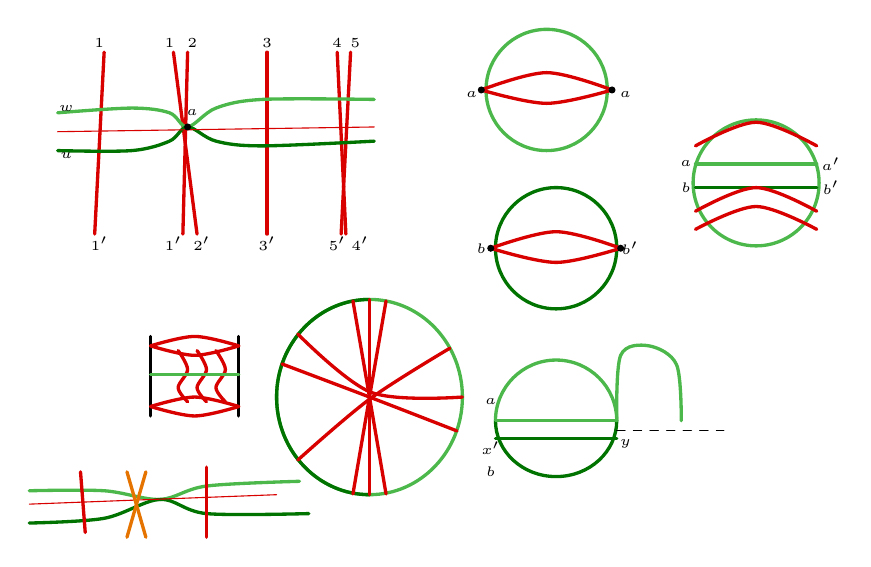
\begin{tikzpicture}[x=1mm,y=1mm,line cap=round,line join=round,font=\scriptsize]
\draw[Rd,very thick] (9.5,-11.8) -- (8.3,-34.9);
\draw[Rd,very thick] (18.3,-11.8) -- (21.3,-34.9);
\draw[Rd,very thick] (20.1,-11.8) -- (19.5,-34.9);
\draw[Rd,very thick] (30.2,-11.8) -- (30.2,-34.9);
\draw[Rd,very thick] (39.1,-11.8) -- (40.2,-34.9);
\draw[Rd,very thick] (40.8,-11.8) -- (39.6,-34.9);
\draw[Lg,very thick] plot[smooth, tension=0.55] coordinates {(3.6,-19.5) (13,-18.9) (17.8,-19.5) (20.1,-21.3) (23.7,-18.9) (29.6,-17.8) (43.8,-17.8)};
\draw[Dg,very thick] plot[smooth, tension=0.55] coordinates {(3.6,-24.3) (13,-24.3) (17.8,-23.1) (20.1,-21.3) (23.7,-23.1) (29.6,-23.7) (43.8,-23.1)};
\draw[Rd] (3.6,-21.9) -- (43.8,-21.3);
\node[pt] at (20.1,-21.3) {};
\node[inner sep=1pt] at (20.7,-19.5) {\tiny $a$};
\node[inner sep=1pt] at (4.7,-18.9) {\tiny $w$};
\node[inner sep=1pt] at (4.7,-24.9) {\tiny $u$};
\node[inner sep=1pt] at (8.9,-10.7) {\tiny $1$};
\node[inner sep=1pt] at (17.8,-10.7) {\tiny $1$};
\node[inner sep=1pt] at (20.7,-10.7) {\tiny $2$};
\node[inner sep=1pt] at (30.2,-10.7) {\tiny $3$};
\node[inner sep=1pt] at (39.1,-10.7) {\tiny $4$};
\node[inner sep=1pt] at (41.4,-10.7) {\tiny $5$};
\node[inner sep=1pt] at (8.9,-36.1) {\tiny $1'$};
\node[inner sep=1pt] at (18.3,-36.1) {\tiny $1'$};
\node[inner sep=1pt] at (21.9,-36.1) {\tiny $2'$};
\node[inner sep=1pt] at (30.2,-36.1) {\tiny $3'$};
\node[inner sep=1pt] at (39.1,-36.1) {\tiny $5'$};
\node[inner sep=1pt] at (42,-36.1) {\tiny $4'$};
\draw[Lg,very thick] (65.7,-16.6) circle[radius=7.7];
\draw[Rd,very thick] plot[smooth, tension=0.55] coordinates {(57.4,-16.6) (65.7,-14.4) (74,-16.6)};
\draw[Rd,very thick] plot[smooth, tension=0.55] coordinates {(57.4,-16.6) (65.7,-18.3) (74,-16.6)};
\node[pt] at (57.4,-16.6) {};
\node[pt] at (74,-16.6) {};
\node[inner sep=1pt] at (56.2,-17.2) {\tiny $a$};
\node[inner sep=1pt] at (75.7,-17.2) {\tiny $a$};
\draw[Dg,very thick] (66.9,-36.7) circle[radius=7.7];
\draw[Rd,very thick] plot[smooth, tension=0.55] coordinates {(58.6,-36.7) (66.9,-34.6) (75.1,-36.7)};
\draw[Rd,very thick] plot[smooth, tension=0.55] coordinates {(58.6,-36.7) (66.9,-38.5) (75.1,-36.7)};
\node[pt] at (58.6,-36.7) {};
\node[pt] at (75.1,-36.7) {};
\node[inner sep=1pt] at (57.4,-36.7) {\tiny $b$};
\node[inner sep=1pt] at (76.3,-36.7) {\tiny $b'$};
\draw[Lg,very thick] (92.3,-28.4) circle[radius=8];
\draw[Lg,very thick] (84.6,-26) -- (100,-26);
\draw[Dg,very thick] (84.6,-29) -- (100,-29);
\draw[Rd,very thick] plot[smooth, tension=0.55] coordinates {(84.6,-23.7) (92.3,-20.7) (100,-23.7)};
\draw[Rd,very thick] plot[smooth, tension=0.55] coordinates {(84.6,-32) (92.3,-29) (100,-32)};
\draw[Rd,very thick] plot[smooth, tension=0.55] coordinates {(84.6,-34.3) (92.3,-31.4) (100,-34.3)};
\node[inner sep=1pt] at (83.4,-26) {\tiny $a$};
\node[inner sep=1pt] at (101.8,-26) {\tiny $a'$};
\node[inner sep=1pt] at (83.4,-29) {\tiny $b$};
\node[inner sep=1pt] at (101.8,-29) {\tiny $b'$};
\draw[very thick] (15.4,-47.9) -- (15.4,-58);
\draw[very thick] (26.6,-47.9) -- (26.6,-58);
\draw[Rd,very thick] plot[smooth, tension=0.55] coordinates {(15.4,-49.1) (21,-47.9) (26.6,-49.1)};
\draw[Rd,very thick] plot[smooth, tension=0.55] coordinates {(15.4,-49.1) (21,-50.3) (26.6,-49.1)};
\draw[Rd,very thick] plot[smooth, tension=0.55] coordinates {(15.4,-56.8) (21,-55.6) (26.6,-56.8)};
\draw[Rd,very thick] plot[smooth, tension=0.55] coordinates {(15.4,-56.8) (21,-58) (26.6,-56.8)};
\draw[Rd,very thick] plot[smooth, tension=0.55] coordinates {(18.9,-49.7) (20.1,-52.1) (18.9,-54.4) (20.1,-56.2)};
\draw[Rd,very thick] plot[smooth, tension=0.55] coordinates {(21.3,-49.7) (22.5,-52.1) (21.3,-54.4) (22.5,-56.2)};
\draw[Rd,very thick] plot[smooth, tension=0.55] coordinates {(23.7,-49.7) (24.9,-52.1) (23.7,-54.4) (24.9,-56.2)};
\draw[Lg,very thick] (15.4,-52.7) -- (26.6,-52.7);
\draw[Lg,very thick] (43.2,-55.6) ellipse[x radius=11.8, y radius=12.4];
\draw[Dg,very thick] (43.2,-43.2) arc[start angle=90, end angle=270, x radius=11.8, y radius=12.4];
\draw[Rd,very thick] plot[smooth, tension=0.55] coordinates {(43.2,-43.2) (43.2,-55.6) (43.2,-68)};
\draw[Rd,very thick] plot[smooth, tension=0.55] coordinates {(41.1,-43.4) (43.2,-55.6) (45.3,-67.9)};
\draw[Rd,very thick] plot[smooth, tension=0.55] coordinates {(45.3,-43.4) (43.2,-55.6) (41.1,-67.9)};
\draw[Rd,very thick] plot[smooth, tension=0.55] coordinates {(32.1,-51.4) (43.2,-55.6) (54.3,-59.9)};
\draw[Rd,very thick] plot[smooth, tension=0.55] coordinates {(53.4,-49.4) (43.3,-55.8) (34.1,-63.6)};
\draw[Rd,very thick] plot[smooth, tension=0.55] coordinates {(34.1,-47.6) (43.4,-55) (55,-55.6)};
\draw[Lg,very thick] (74.6,-58.6) arc[start angle=0, end angle=180, x radius=7.7, y radius=7.7];
\draw[Dg,very thick] (59.2,-58.6) arc[start angle=180, end angle=360, x radius=7.7, y radius=7.1];
\draw[Lg,very thick] (59.2,-58.6) -- (74.6,-58.6);
\draw[Dg,very thick] (59.2,-60.9) -- (74.6,-60.9);
\draw[Lg,very thick] plot[smooth, tension=0.55] coordinates {(74.6,-58.6) (75.1,-50.3) (78.7,-49.1) (82.2,-51.5) (82.8,-58.6)};
\draw[dashed] (74.6,-59.8) -- (88.2,-59.8);
\node[inner sep=1pt] at (58.6,-56.2) {\tiny $a$};
\node[inner sep=1pt] at (58.6,-62.1) {\tiny $x'$};
\node[inner sep=1pt] at (58.6,-65.1) {\tiny $b$};
\node[inner sep=1pt] at (75.7,-61.5) {\tiny $y$};
\draw[Lg,very thick] plot[smooth, tension=0.55] coordinates {(0,-67.5) (9.5,-67.5) (16.6,-68.6) (22.5,-66.9) (34.3,-66.3)};
\draw[Dg,very thick] plot[smooth, tension=0.55] coordinates {(0,-71.6) (9.5,-71) (16.6,-68.6) (22.5,-70.4) (35.5,-70.4)};
\draw[Rd] (0,-69.2) -- (31.4,-68);
\draw[Rd,very thick] (6.5,-65.1) -- (7.1,-72.8);
\draw[Or,very thick] (12.4,-65.1) -- (14.8,-73.4);
\draw[Or,very thick] (14.8,-65.1) -- (12.4,-73.4);
\draw[Rd,very thick] (22.5,-64.5) -- (22.5,-73.4);
\end{tikzpicture}
\end{document}
